\chapter{Wire Equivalency Protocol (WEP)}
\label{ch:wep}

\section{WEP Einführung}
Als erstes, weit verbreitetes Sicherheitsprotokoll hat sich \acrfull{wepLabel} durchgesetzt.
Trotzdem, dass \gls{wepLabel} grosse Schwachstellen und Sicherheitslücken aufweist und diese seit langem (2001) auch bekannt sind, wird \gls{wepLabel} immer noch angewendet (einerseits von alten Geräten, aber auch neue, die aus Kompatibilitätsgründen verschiedene Sicherheitsprotokolle anbieten).
Da \gls{wepLabel} als veraltet gilt und offiziell abgelöst wurde, wird nicht genau auf technische Einzelheiten eingegangen.

Der Schlüssel ist theoretisch 64 oder 128 Bits lang.
Da davon jedoch 24 Bits für den \gls{ivLabel} verwendet werde, und der unverschlüsselt übermittelt wird, kürzt sich die Schlüssellänge erheblich.
Sprich die effektive Länge des Schlüssel ist 40 oder 104 Bits.
%Die verkürzte Schlüssellänge ist jedoch nicht das Hauptproblem von \gls{wepLabel}.

\section{Angriff auf WEP}
Nebst fehlerhaften \gls{wepLabel} Implementationen konkreter Hersteller, können allgemeine \gls{wepLabel}-Angriffe in zwei Kategorien eingeteilt werden.\footcite[][126f.]{WrightCache201503}:
In Netzwerke mit aktiven Clients (und entsprechendem Datenverkehr) und solche ohne aktive Clients.

\subsection{Angriff mit einem Opfer Client (WEP)}
Der Angriff auf ein Netzwerk mit Clients ist einfacher, kann jedoch mehr Geduld beanspruchen.

Ein durchgeführtes Beispiel ist im \secref{sec:wepAttack} dokumentiert.


\subsection{Angriff ohne einem Opfer Client (WEP)}
Ein Angriff auf ein Netzwerk ohne Clients ist aufwändiger.
Die notwendigen Schritten des Angriffes werden kurz erläutert:\footcite[][129f.]{WrightCache201503}
\begin{enumerate}
	\item Daten eines Channels aufzeichnen\\
	\texttt{airodump-ng} (ergibt eine \textit{*.cap} Datei)

	\item erfolgreiche Verbindung vortäuschen\\
	\texttt{aireplay-ng  -{}-fakeauth}

	\item \textit{Fragmentation-} oder \textit{ChopChop-Angriff}\\
	\texttt{(aireplay-ng -{}-fragment)} oder \texttt{(aireplay-ng -{}-chopchop)}

	\item Eigenes broadcast \gls{arpLabel} Paket bauen\\
	\texttt{packetforge-ng -{}-arp}

	\item \gls{arpLabel} an \gls{apLabel} senden (inject)\\
	\texttt{aireplay-ng -{}-interactive}

	\item Aufzeichnung von Schritt 1 knacken\\
	\texttt{aircrack-ng}

\end{enumerate}

\begin{framed}
	\textbf{Bemerkung:} Dieser Angriff wurde nicht durchgeführt, da das \textit{inject} (senden eines selbst gebauten Paketes) nur von speziellen Netzwerkkarten unterstützt wird.\footcite[][89f.]{WrightCache201503}
	Zu jenen die des \textit{Mac Book Air's} nicht gehört.
\end{framed}


\subsection{Konkreter Angriff auf ein WEP-Netzwerk mit einem Opfer Client}
\label{sec:wepAttack}
Folgend wird ein erfolgreicher Angriff auf ein \gls{wepLabel}-Netzwerk durchgeführt.

\subsection{Setup}
\subsubsection{Hardware}
Nebst der in \secref{sec:testEnvroiment} beschriebene Hardware wurde ein ältere Swisscom Router \textit{Netopia  3357NWG}\footcite{Netopia_3347_57nwg_de_2015-04-06} verwendet. Der Router wurde mit einem 10-stelligen hexadezimalen \gls{pskLabel} eingerichtet.

\subsection{Ausführung}
\label{subsec:wep_crack_tutorial}
Mit dem "`Wireless Diagnostics"' Tool von Apple kann via \textit{Window} $\rightarrow$ das \textit{Scan} und das \textit{Sniffer} Programm geöffnet werden.
Mit dem \textit{Scan} Programm können verfügbare Netze und deren Channels gefunden werden.

\begin{figure}[H]
	\centering
	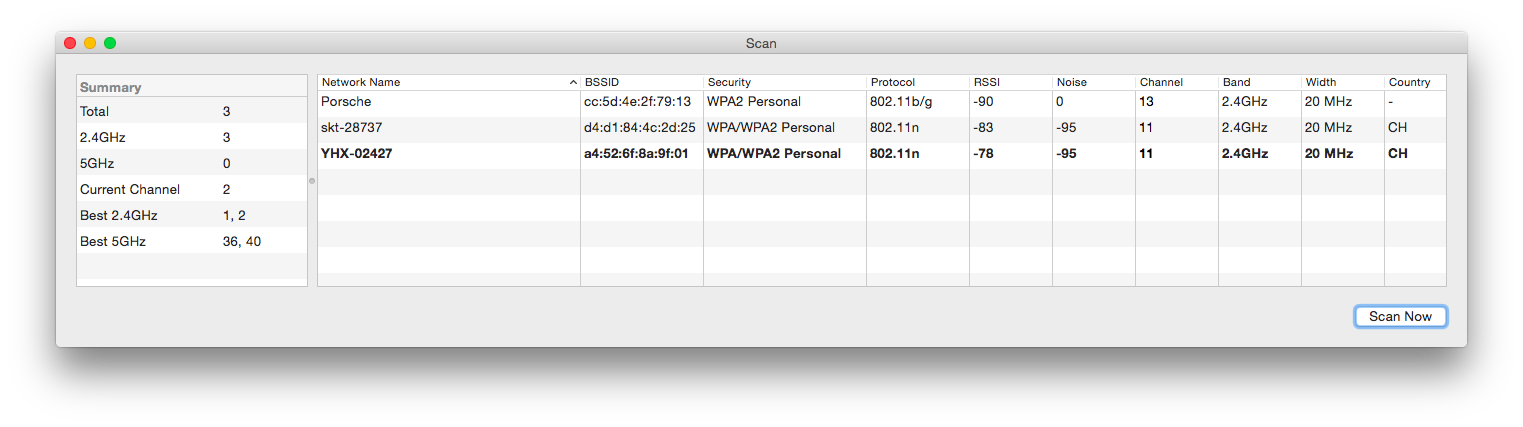
\includegraphics[width=1.0\textwidth]{images/wep/scan.png}
	\caption{OS X Wireless Diagnostics: Scanner}
\end{figure}

Mit dem \textit{Sniffer} können benötigte Daten aus einem konkreten Netz aufgezeichnet werden. Es werden ca. 5'000 \gls{ivLabel}'s benötigt um den Schlüssel zu berechnen. Eine solche Aufzeichnung (capture) dauert unterschiedlich lange, je nach Nutzung des Netzes. Wird das Netz viel gebraucht, geht es schneller.

\begin{figure}[H]
	\centering
	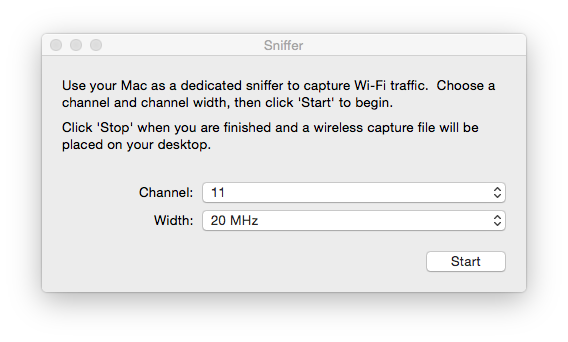
\includegraphics[width=0.8\textwidth]{images/wep/sniffer.png}
	\caption{OS X Wireless Diagnostics: Sniffer}
\end{figure}

%\begin{wrapfigure}{r}{0.6\textwidth}
%	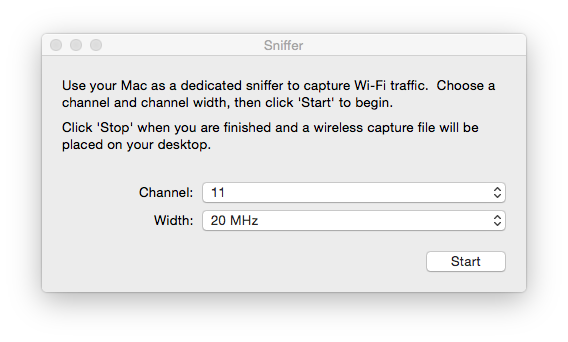
\includegraphics[width=1.0\linewidth]{images/wep/sniffer.png}
%	\caption{OS X Wireless Diagnostics: Sniffer}
%\end{wrapfigure}

Der Sniffer kann auch direkt über die Kommandozeile ausgeführt werden:
\begin{lstlisting}[style=lstStyleFramed]
sudo ln -s /System/Library/PrivateFrameworks/Apple80211.framework/Versions/Current/Resources/airport /usr/sbin/airport
sudo airport en0 sniff <CHANNEL>
\end{lstlisting}

Anschliessend können die Daten, vom \textit{Sniffer} mit dem \textit{aircrack-ng} ausgewertet werden:
\begin{lstlisting}[style=lstStyleFramed]
aircrack-ng -b 00:0f:cc:b0:1a:c8 /private/tmp/airportSniff*.cap
\end{lstlisting}

So wird einem, falls genügend \gls{ivLabel}'s vorhanden sind, der \gls{wepLabel} ausgegeben (Dauer: 2 Sek.).
\begin{figure}[H]
	\centering
	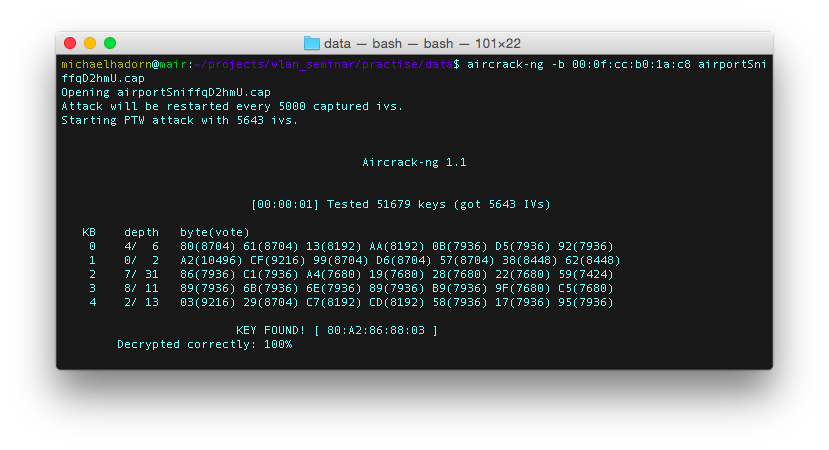
\includegraphics[width=1.0\textwidth]{images/wep/aircrack-ng.png}
	\caption[aircrack-ng: WEP Schlüssel knacken -- Terminalausgabe]{aircrack-ng: \gls{wepLabel} Schlüssel knacken -- Terminalausgabe}
\end{figure}
